\documentclass[12pt]{article}
\usepackage[a4paper,margin=2.5cm]{geometry}
\usepackage{tikz}
\usepackage{xcolor}
\usetikzlibrary{angles,quotes}
\definecolor{goldenrod}{RGB}{201,162,39}

\begin{document}

\section*{Segitiga dengan Tiga Sudutnya}

% Segitiga ABC: A=(0,0), B=(5,0), C=(1.8,3.2).
% Sudut A = 61 derajat, sudut B = 45 derajat, sudut C = 74 derajat.
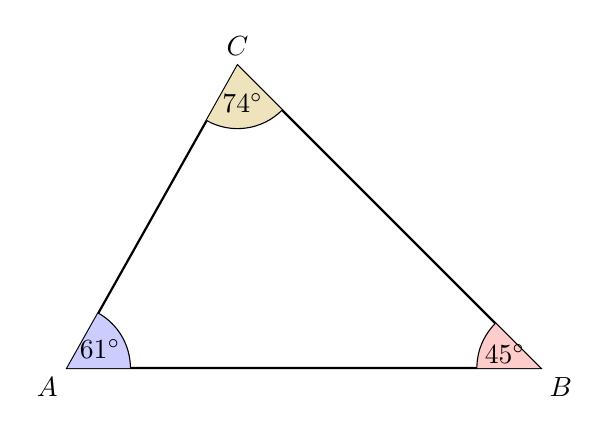
\begin{tikzpicture}[scale=1.2]
  \coordinate (A) at (0,0);
  \coordinate (B) at (5,0);
  \coordinate (C) at (1.8,3.2);
  % Segitiga
  \draw[thick] (A) -- (B) -- (C) -- cycle;
  % Nama titik sudut
  \node[below left] at (A) {$A$};
  \node[below right] at (B) {$B$};
  \node[above] at (C) {$C$};
  % Tanda sudut dengan warnanya masing-masing
  \pic[draw, fill=blue!20, angle radius=0.8cm, "$61^\circ$"] {angle = B--A--C};
  \pic[draw, fill=red!20, angle radius=0.8cm, "$45^\circ$"] {angle = C--B--A};
  \pic[draw, fill=goldenrod!30, angle radius=0.8cm, "$74^\circ$"] {angle = A--C--B};
\end{tikzpicture}

\section*{Ketiga Sudut Dijajarkan pada Satu Garis Lurus}

% Juring-juring 61, 45, dan 74 derajat yang dijajarkan di atas satu garis.
% Batas-batasnya pada sudut 180, 119, 74, dan 0 derajat, jari-jari 1,8 cm.
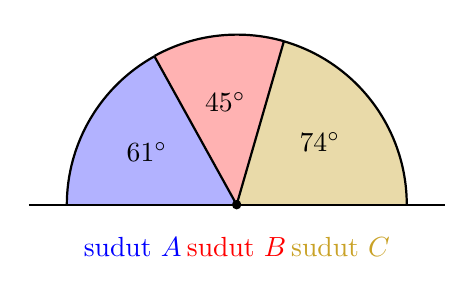
\begin{tikzpicture}[scale=1.2]
  \coordinate (O) at (0,0);
  \coordinate (P180) at (-1.8,0);
  \coordinate (P119) at (-0.87,1.57);
  \coordinate (P74) at (0.50,1.73);
  \coordinate (P0) at (1.8,0);
  % Garis lurus tempat ketiga sudut dijajarkan
  \draw[thick] (-2.2,0) -- (2.2,0);
  % Juring sudut A: 61 derajat (dari 119 ke 180 derajat)
  \fill[blue!30] (O) -- (P119) arc (119:180:1.8) -- cycle;
  % Juring sudut B: 45 derajat (dari 74 ke 119 derajat)
  \fill[red!30] (O) -- (P74) arc (74:119:1.8) -- cycle;
  % Juring sudut C: 74 derajat (dari 0 ke 74 derajat)
  \fill[goldenrod!40] (O) -- (P0) arc (0:74:1.8) -- cycle;
  % Busur-busur pembatas juring
  \draw[thick] (O) -- (P180);
  \draw[thick] (O) -- (P119);
  \draw[thick] (O) -- (P74);
  \draw[thick] (O) -- (P0);
  \draw[thick] (P119) arc (119:180:1.8);
  \draw[thick] (P74) arc (74:119:1.8);
  \draw[thick] (P0) arc (0:74:1.8);
  % Titik pusat dan label sudut
  \fill (O) circle (0.05);
  \node at (-0.95,0.56) {$61^\circ$};
  \node at (-0.12,1.09) {$45^\circ$};
  \node at (0.88,0.66) {$74^\circ$};
  % Keterangan warna
  \node[blue] at (-1.1,-0.45) {sudut $A$};
  \node[red] at (0,-0.45) {sudut $B$};
  \node[goldenrod] at (1.1,-0.45) {sudut $C$};
\end{tikzpicture}

\end{document}
